\documentclass[12pt]{article}
\usepackage{fullpage}
\usepackage{titlesec}
\usepackage{tikz}
\usepackage{amsfonts,amssymb}
\usepackage{amsmath}
\usepackage{comment}
\usepackage{multicol}
\usetikzlibrary{automata, positioning}

\input ../libraries/mac.tex
\input ../libraries/mathmac.tex

\begin{document}
\pagestyle{plain}
\titleformat{\subsection}[runin]
  {\normalfont\large\bfseries}{\thesubsection}{1em}{}

\title{Homework 4}
\author{Brooke Fugate, Michael O'Connor, Rohan Shah}
\date{}

\maketitle

\section*{Problem B6}
\subsection*{(1)}
\begin{center}
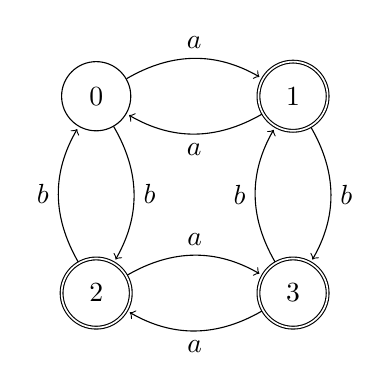
\begin{tikzpicture}[shorten >=1pt, node distance=2.5cm, on grid, auto]
  \node[state] (q0) {0};
  \node[state, accepting] (q1) [right=of q0] {1};
  \node[state, accepting] (q2) [below=of q0] {2};
  \node[state, accepting] (q3) [right =of q2] {3};
  \path[->]
(q0) edge [bend left] node {$a$} (q1)
(q0) edge [bend left] node {$b$} (q2)
(q1) edge [bend left] node {$a$} (q0)
(q1) edge [bend left] node {$b$} (q3)
(q2) edge [bend left] node {$a$} (q3)
(q2) edge [bend left] node {$b$} (q0)
(q3) edge [bend left] node {$a$} (q2)
(q3) edge [bend left] node {$b$} (q1)
  ;
\end{tikzpicture}
\end{center}

\subsection*{(2)}
$(\epsilon +(a+b)(bb+(a+b)(a+b))^*(\epsilon +a+b))+
((\epsilon +a+b)+(a+b)(bb+(a+b)(a+b))^*(ba+(a+b)(a+b)))
((aa+(a+b)(a+b)+(ab+(a+b)(a+b))(bb+(a+b)(a+b))^*(ba+(a+b)(a+b)))^*
((a+b)+(ab+(a+b)(a+b))(bb+(a+b)(a+b))^*(\epsilon+a+b))$

\subsubsection*{Node Elimination Steps:}
\textbf{Initial Edges}
\begin{multicols}{4}
\noindent
$(0,1) = a$\\
$(0,2) = b$\\
\columnbreak
\break
$(1,0) = a$\\
$(1,3) = b$\\
\columnbreak
\break
$(2,0) = b$\\
$(2,3) = a$\\
\columnbreak
\break
$(3,1) = b$\\
$(3,2) = a$\\
\end{multicols}

\noindent\textbf{After Preprocessing}
\begin{multicols}{5}
\noindent
$(s,0) = \epsilon$\\
$(s,1) = \emptyset$\\
$(s,2) = \emptyset$\\
$(s,3) = \emptyset$\\
$(s,t) = \emptyset$\\
\columnbreak
\break
$(0,0) = \emptyset$\\
$(0,1) = a$\\
$(0,2) = b$\\
$(0,3) = \emptyset$\\
$(0,t) = \emptyset$\\
\columnbreak
\break
$(1,0) = a$\\
$(1,1) = \emptyset$\\
$(1,2) = \emptyset$\\
$(1,3) = b$\\
$(1,t) = \epsilon$\\
\columnbreak
\break
$(2,0) = b$\\
$(2,1) = \emptyset$\\
$(2,2) = \emptyset$\\
$(2,3) = a$\\
$(2,t) = \epsilon$\\
\columnbreak
\break
$(3,0) = \emptyset$\\
$(3,1) = b$\\
$(3,2) = a$\\
$(3,3) = \emptyset$\\
$(3,t) = \epsilon$\\
\end{multicols}

\noindent\textbf{After Eliminating Node 1}
\begin{multicols}{4}
\noindent
$(s,0) = \epsilon + a$\\
$(s,2) = \emptyset$\\
$(s,3) = \emptyset + b$\\
$(s,t) = \epsilon$\\
\columnbreak
\break
$(0,0) = aa$\\
$(0,2) = b+a$\\
$(0,3) = ab$\\
$(0,t) = a$\\
\columnbreak
\break
$(2,0) = b+a$\\
$(2,2) = \emptyset$\\
$(2,3) = a+b$\\
$(2,t) = \epsilon$\\
\columnbreak
\break
$(3,0) = ba$\\
$(3,2) = a+b$\\
$(3,3) = b$\\
$(3,t) = \epsilon+b$\\
\end{multicols}

\noindent\textbf{After Eliminating Node 2}
\begin{multicols}{3}
\noindent
$(s,0) = (\epsilon + a+b)$\\
$(s,3) = (a+b)$\\
$(s,t) = \epsilon$\\
\columnbreak
\break
$(0,0) = (aa+(b+a)(b+a))$\\
$(0,3) = (ab+(b+a)(a+b))$\\
$(0,t) = (a+b)$\\
\columnbreak
\break
$(3,0) = (ba+(a+b)(b+a))$\\
$(3,3) = (b+(a+b)(a+b))$\\
$(3,t) = ((\epsilon+b)+(a+b)(\epsilon + b))$\\
\end{multicols}

\noindent\textbf{After Eliminating Node 3}\\
$(s,0) = ((\epsilon + a+b) + (a+b)(b+(a+b)(a+b))^*(ba+(a+b)(b+a)))$\\
$(s,t) = (\epsilon + (a+b)(b+(a+b)(a+b))^*((\epsilon+b)+(a+b)(\epsilon + b)))$\\
$(0,0) = ((aa+(b+a)(b+a)) + (ab+(b+a)(a+b))(b+(a+b)(a+b))^*(ba+(a+b)(b+a)))$\\
$(0,t) = ((a+b) + (ab+(b+a)(a+b))(b+(a+b)(a+b))^*((\epsilon+b)+(a+b)(\epsilon + b)))$\\

\noindent\textbf{After Eliminating Node 0}\\
$(s,t) = (\epsilon + (a+b)(b+(a+b)(a+b))^*((\epsilon+b)+(a+b)(\epsilon + b))) +
((\epsilon + a+b) + (a+b)(b+(a+b)(a+b))^*(ba+(a+b)(b+a)))
((aa+(b+a)(b+a)) + (ab+(b+a)(a+b))(b+(a+b)(a+b))^*(ba+(a+b)(b+a)))^*
((a+b) + (ab+(b+a)(a+b))(b+(a+b)(a+b))^*((\epsilon+b)+(a+b)(\epsilon + b)))
$\\

\end{document}
